

\section{Introduction}
\label{sec:intro}


A central problem in sequence modeling is efficiently handling data that contains long-range dependencies (LRDs).
Real-world time-series data often requires reasoning over tens of thousands of time steps, while few sequence models address even thousands of time steps.
For instance, results from the long-range arena (LRA) benchmark~\citep{tay2021long} highlight that sequence models today perform poorly on LRD tasks,
including one (Path-X) where no model performs better than random guessing.










\begin{figure}[!t]
    \centering
    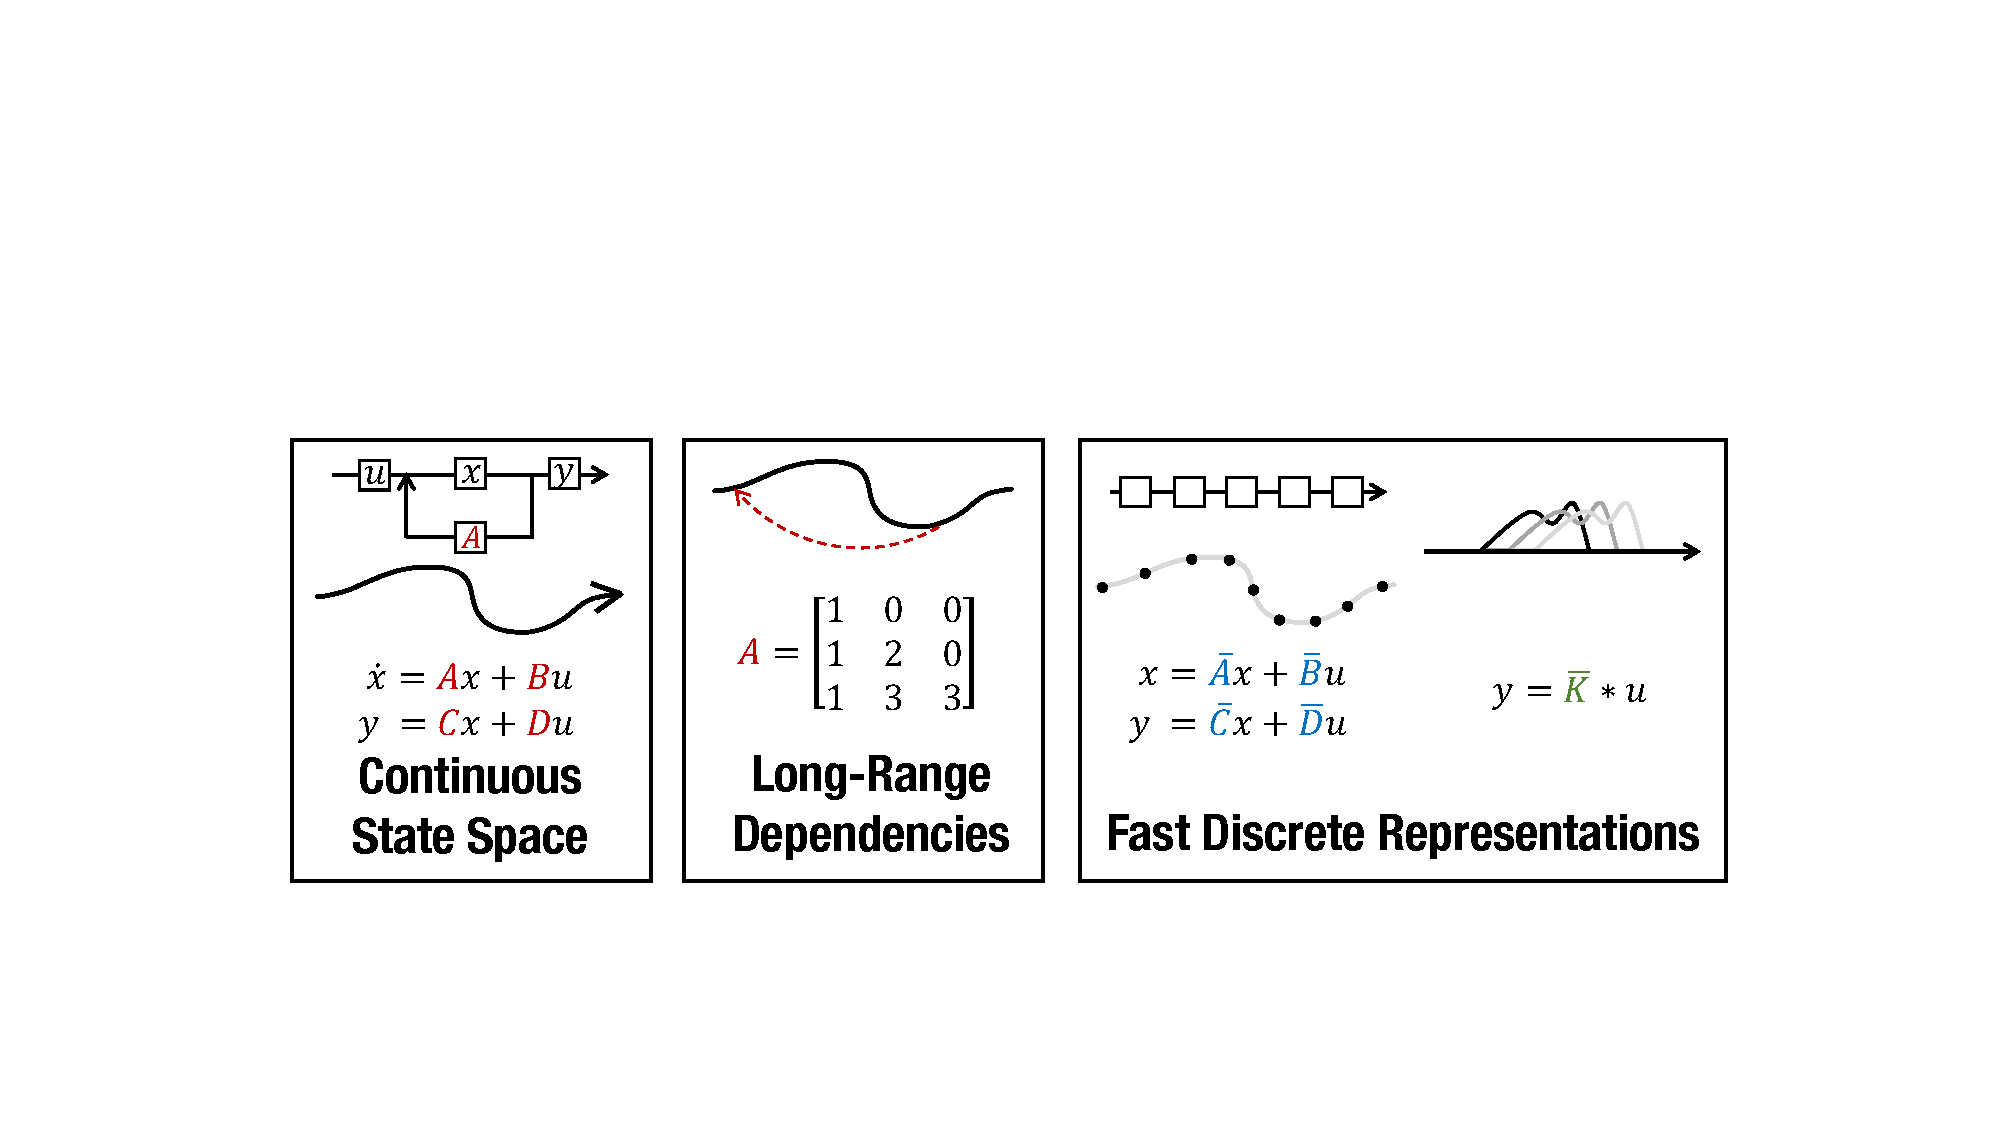
\includegraphics[width=\linewidth]{figs/properties.pdf}
    \caption{
      (\textbf{Left}) State Space Models (SSM) parameterized by matrices \( \bm{A}, \bm{B}, \bm{C}, \bm{D} \) map an input signal \( u(t) \) to output \( y(t) \) through a latent state \( x(t) \).
      (\textbf{Center}) Recent theory on continuous-time memorization derives special \( \bm{A} \) matrices that allow SSMs to capture LRDs mathematically and empirically.
      (\textbf{Right}) SSMs can be computed either as a recurrence (left) or convolution (right).
      However, materializing these conceptual views requires utilizing different representations of its parameters (\textcolor{BrickRed}{red}, \textcolor{RoyalBlue}{blue}, \textcolor{ForestGreen}{green}) which are very expensive to compute.
      \methodabbrv{} introduces a novel parameterization that efficiently swaps between these representations, allowing it to handle a wide range of tasks, be efficient at both training and inference, and excel at long sequences.
    }
\label{fig:properties}
\end{figure}


Since LRDs are perhaps {the} foremost challenge for sequence models, all standard model families such as continuous-time models (CTMs), RNNs, CNNs, and Transformers include many specialized variants designed to address them.
Modern examples include orthogonal and Lipschitz RNNs \citep{arjovsky2016unitary,erichson2021lipschitz} to combat vanishing gradients, dilated convolutions to increase context size \citep{bai2018empirical,oord2016wavenet}, and an increasingly vast family of efficient Transformers that reduce the quadratic dependence on sequence length \citep{katharopoulos2020transformers,choromanski2020rethinking}.
Despite being designed for LRDs, these solutions still perform poorly on challenging benchmarks such as LRA~\citep{tay2021long} or raw audio classification~\citep{gu2021lssl}.


An alternative approach to LRDs was recently introduced based on the \textbf{state space model (SSM)} (\cref{fig:properties}).
SSMs are a foundational scientific model used in fields such as control theory, computational neuroscience, and many more, but have not been applicable to deep learning for concrete theoretical reasons.
In particular, \citet{gu2021lssl} showed that deep SSMs actually struggle even on simple tasks,
but can perform exceptionally well when equipped with special state matrices \( \bm{A} \) recently derived to solve a problem of continuous-time memorization \citep{voelker2019legendre,gu2020hippo}.
Their Linear State Space Layer (LSSL) conceptually unifies the strengths of CTM, RNN and CNN models, and provides a proof of concept that deep SSMs can address LRDs in principle.

Unfortunately, the LSSL is infeasible to use in practice because of prohibitive computation and memory requirements induced by the state representation.
For state dimension \( N \) and sequence length \( L \), computing the latent state requires \( O(N^2L) \) operations and \( O(NL) \) space -- compared to a \( \Omega(L+N) \) lower bound for both.
Thus for reasonably sized models (e.g. \( N=256 \) in \citet{gu2021lssl}), the LSSL uses orders of magnitude more memory than comparably-sized RNNs or CNNs.
Although theoretically efficient algorithms for the LSSL were proposed, we show that these are numerically unstable.
In particular, the special \( \bm{A} \) matrix is highly non-normal in the linear algebraic sense, which prevents the application of conventional algorithmic techniques. %
Consequently, although the LSSL showed that SSMs have strong performance, they are currently computationally impractical as a general sequence modeling solution.

In this work, we introduce the \textbf{Structured State Space (\methodabbrv)} sequence model based on the SSM that solves the critical computational bottleneck in previous work.
Technically, \methodabbrv{} reparameterizes the structured state matrices \( \bm{A} \) appearing in \citet{voelker2019legendre,gu2020hippo} by decomposing them as the sum of a low-rank and normal term.
Additionally, instead of expanding the standard SSM in coefficient space, we compute its truncated generating function in frequency space, which can be simplified into a multipole-like evaluation.
Combining these two ideas, we show that the low-rank term can be corrected by the Woodbury identity while the normal term can be diagonalized stably,
ultimately reducing to a well-studied and theoretically stable Cauchy kernel \citep{pan2001structured,pan2017fast}.
This results in \( \tilde{O}(N+L) \) computation and \( O(N+L) \) memory usage, which is essentially tight for sequence models.
Compared to the LSSL, \methodabbrv{} is up to $30\times$ faster with $400\times$ less memory usage, while exceeding the LSSL's performance empirically.






Empirically, \methodabbrv{} significantly advances the state-of-the-art for LRD.
On the LRA benchmark for efficient sequence models, \methodabbrv{} is as fast as all baselines while outperforming them by $20+$ points on average.
\methodabbrv{} is the first model to solve the difficult LRA Path-X task (length-$16384$), achieving \textbf{88\% accuracy compared to 50\% random guessing} for all prior work.
On speech classification with length-$16000$ sequences, \methodabbrv{} halves the test error ($1.7\%$) of specialized Speech CNNs --
by contrast, all RNN and Transformer baselines fail to learn ($\ge 70\%$ error).



\paragraph{Towards a general-purpose sequence model.}
Beyond LRD, a broad goal of machine learning is to develop a single model that can be used across a wide range of problems.
Models today are typically specialized to solve problems from a particular domain (e.g. images, audio, text, time-series), and enable a narrow range of capabilities (e.g. efficient training, fast generation, handling irregularly sampled data).
This specialization is typically expressed via domain-specific preprocessing, inductive biases, and architectures. %
Sequence models provide a general framework for solving many of these problems with reduced specialization
-- e.g. Vision Transformers for image classification with less 2D information \citep{dosovitskiy2020image}. %
However, most models such as Transformers generally still require substantial specialization per task to achieve high performance.





Deep SSMs in particular have conceptual strengths that suggest they may be promising as a general sequence modeling solution.
These strengths include a principled approach to handling LRDs, as well as the ability to move between continuous-time, convolutional, and recurrent model representations, each with distinct capabilities (\cref{fig:properties}). %
Our technical contributions enable SSMs to be applied successfully to a varied set of benchmarks with minimal modification: %
\begin{itemize}[leftmargin=*]
    \item {\it Large-scale generative modeling.}
        On CIFAR-10 density estimation, \methodabbrv{} is competitive with the best autoregressive models ($2.85$ bits per dim). On WikiText-103 language modeling, \methodabbrv{} substantially closes the gap to Transformers (within $0.8$ perplexity), setting SoTA for attention-free models.
    \item {\it Fast autoregressive generation.}
        Like RNNs, \methodabbrv{} can use its latent state to perform $60\times$ faster pixel/token generation than standard autoregressive models on CIFAR-10 and WikiText-103.
    \item {\it Sampling resolution change.}
        Like specialized CTMs, \methodabbrv{} can adapt to changes in time-series sampling frequency without retraining, e.g.\ at $0.5\times$ frequency on speech classification.
    \item {\it Learning with weaker inductive biases.}
        With no architectural changes, \methodabbrv{} surpasses Speech CNNs on speech classification, outperforms the specialized Informer model on time-series forecasting problems,
        and matches a 2-D ResNet on sequential CIFAR with over $90\%$ accuracy.



\end{itemize}









